\documentclass[journal, a4paper]{IEEEtran}

% some very useful LaTeX packages include:

%\usepackage{cite}      % Written by Donald Arseneau
                        % V1.6 and later of IEEEtran pre-defines the format
                        % of the cite.sty package \cite{} output to follow
                        % that of IEEE. Loading the cite package will
                        % result in citation numbers being automatically
                        % sorted and properly "ranged". i.e.,
                        % [1], [9], [2], [7], [5], [6]
                        % (without using cite.sty)
                        % will become:
                        % [1], [2], [5]--[7], [9] (using cite.sty)
                        % cite.sty's \cite will automatically add leading
                        % space, if needed. Use cite.sty's noadjust option
                        % (cite.sty V3.8 and later) if you want to turn this
                        % off. cite.sty is already installed on most LaTeX
                        % systems. The latest version can be obtained at:
                        % http://www.ctan.org/tex-archive/macros/latex/contrib/supported/cite/

\usepackage{graphicx}   % Written by David Carlisle and Sebastian Rahtz
                        % Required if you want graphics, photos, etc.
                        % graphicx.sty is already installed on most LaTeX
                        % systems. The latest version and documentation can
                        % be obtained at:
                        % http://www.ctan.org/tex-archive/macros/latex/required/graphics/
                        % Another good source of documentation is "Using
                        % Imported Graphics in LaTeX2e" by Keith Reckdahl
                        % which can be found as esplatex.ps and epslatex.pdf
                        % at: http://www.ctan.org/tex-archive/info/

%\usepackage{psfrag}    % Written by Craig Barratt, Michael C. Grant,
                        % and David Carlisle
                        % This package allows you to substitute LaTeX
                        % commands for text in imported EPS graphic files.
                        % In this way, LaTeX symbols can be placed into
                        % graphics that have been generated by other
                        % applications. You must use latex->dvips->ps2pdf
                        % workflow (not direct pdf output from pdflatex) if
                        % you wish to use this capability because it works
                        % via some PostScript tricks. Alternatively, the
                        % graphics could be processed as separate files via
                        % psfrag and dvips, then converted to PDF for
                        % inclusion in the main file which uses pdflatex.
                        % Docs are in "The PSfrag System" by Michael C. Grant
                        % and David Carlisle. There is also some information
                        % about using psfrag in "Using Imported Graphics in
                        % LaTeX2e" by Keith Reckdahl which documents the
                        % graphicx package (see above). The psfrag package
                        % and documentation can be obtained at:
                        % http://www.ctan.org/tex-archive/macros/latex/contrib/supported/psfrag/

%\usepackage{subfigure} % Written by Steven Douglas Cochran
                        % This package makes it easy to put subfigures
                        % in your figures. i.e., "figure 1a and 1b"
                        % Docs are in "Using Imported Graphics in LaTeX2e"
                        % by Keith Reckdahl which also documents the graphicx
                        % package (see above). subfigure.sty is already
                        % installed on most LaTeX systems. The latest version
                        % and documentation can be obtained at:
                        % http://www.ctan.org/tex-archive/macros/latex/contrib/supported/subfigure/

\usepackage{url}        % Written by Donald Arseneau
                        % Provides better support for handling and breaking
                        % URLs. url.sty is already installed on most LaTeX
                        % systems. The latest version can be obtained at:
                        % http://www.ctan.org/tex-archive/macros/latex/contrib/other/misc/
                        % Read the url.sty source comments for usage information.

%\usepackage{stfloats}  % Written by Sigitas Tolusis
                        % Gives LaTeX2e the ability to do double column
                        % floats at the bottom of the page as well as the top.
                        % (e.g., "\begin{figure*}[!b]" is not normally
                        % possible in LaTeX2e). This is an invasive package
                        % which rewrites many portions of the LaTeX2e output
                        % routines. It may not work with other packages that
                        % modify the LaTeX2e output routine and/or with other
                        % versions of LaTeX. The latest version and
                        % documentation can be obtained at:
                        % http://www.ctan.org/tex-archive/macros/latex/contrib/supported/sttools/
                        % Documentation is contained in the stfloats.sty
                        % comments as well as in the presfull.pdf file.
                        % Do not use the stfloats baselinefloat ability as
                        % IEEE does not allow \baselineskip to stretch.
                        % Authors submitting work to the IEEE should note
                        % that IEEE rarely uses double column equations and
                        % that authors should try to avoid such use.
                        % Do not be tempted to use the cuted.sty or
                        % midfloat.sty package (by the same author) as IEEE
                        % does not format its papers in such ways.

\usepackage{amsmath}    % From the American Mathematical Society
                        % A popular package that provides many helpful commands
                        % for dealing with mathematics. Note that the AMSmath
                        % package sets \interdisplaylinepenalty to 10000 thus
                        % preventing page breaks from occurring within multiline
                        % equations. Use:
%\interdisplaylinepenalty=2500
                        % after loading amsmath to restore such page breaks
                        % as IEEEtran.cls normally does. amsmath.sty is already
                        % installed on most LaTeX systems. The latest version
                        % and documentation can be obtained at:
                        % http://www.ctan.org/tex-archive/macros/latex/required/amslatex/math/



% Other popular packages for formatting tables and equations include:

%\usepackage{array}
% Frank Mittelbach's and David Carlisle's array.sty which improves the
% LaTeX2e array and tabular environments to provide better appearances and
% additional user controls. array.sty is already installed on most systems.
% The latest version and documentation can be obtained at:
% http://www.ctan.org/tex-archive/macros/latex/required/tools/

% V1.6 of IEEEtran contains the IEEEeqnarray family of commands that can
% be used to generate multiline equations as well as matrices, tables, etc.

% Also of notable interest:
% Scott Pakin's eqparbox package for creating (automatically sized) equal
% width boxes. Available:
% http://www.ctan.org/tex-archive/macros/latex/contrib/supported/eqparbox/

% *** Do not adjust lengths that control margins, column widths, etc. ***
% *** Do not use packages that alter fonts (such as pslatex).         ***
% There should be no need to do such things with IEEEtran.cls V1.6 and later.


% Your document starts here!
\begin{document}
\begin{titlepage}

\newcommand{\HRule}{\rule{\linewidth}{0.5mm}} % Defines a new command for the horizontal lines, change thickness here

\center % Center everything on the page
 %----------------------------------------------------------------------------------------
%	LOGO SECTION
%----------------------------------------------------------------------------------------

~\\[1cm]

\includegraphics{SCUT.png}\\[2cm] % Include a department/university logo - this will require the graphicx package

%----------------------------------------------------------------------------------------
%	TITLE SECTION
%----------------------------------------------------------------------------------------

\HRule \\[1cm]
{ \huge \bfseries The Experiment Report of \textit{Machine Learning} }\\[0.6cm] % Title of your document
\HRule \\[2cm]
%----------------------------------------------------------------------------------------
%	HEADING SECTIONS
%----------------------------------------------------------------------------------------


\textsc{\LARGE \textbf{School:} School of Software Engineering}\\[1cm]
\textsc{\LARGE \textbf{Subject:} Software Engineering}\\[2cm]


%----------------------------------------------------------------------------------------
%	AUTHOR SECTION
%----------------------------------------------------------------------------------------

\begin{minipage}{0.4\textwidth}
\begin{flushleft} \large
\emph{Author:}\\
Haipeng Deng % Your name
\end{flushleft}
\end{minipage}
~
\begin{minipage}{0.4\textwidth}
\begin{flushright} \large
\emph{Supervisor:} \\
Mingkui Tan % Supervisor's Name
\end{flushright}
\end{minipage}\\[2cm]
~
\begin{minipage}{0.4\textwidth}
\begin{flushleft} \large
\emph{Student ID:}\\
201730686193
\end{flushleft}
\end{minipage}
~
\begin{minipage}{0.4\textwidth}
\begin{flushright} \large
\emph{Grade:} \\
Undergraduate
\end{flushright}
\end{minipage}\\[2cm]

% If you don't want a supervisor, uncomment the two lines below and remove the section above
%\Large \emph{Author:}\\
%John \textsc{Smith}\\[3cm] % Your name

%----------------------------------------------------------------------------------------
%	DATE SECTION
%----------------------------------------------------------------------------------------

{\large \today}\\[2cm] % Date, change the \today to a set date if you want to be precise


%----------------------------------------------------------------------------------------

\vfill % Fill the rest of the page with whitespace

\end{titlepage}

% Define document title and author
	\title{Logistic Regression and Support Vector Machine}
	\maketitle

% Write abstract here
\begin{abstract}
This report introduces my work in Lab2 : Logistic Regression and Support Vector Machine. In this lab, a logistic regression model and a SVM are constructed and Mini-Batch Stochastic Gradient Descent is the method of minimizing the loss of the two models.
\end{abstract}

% Each section begins with a \section{title} command
\section{Introduction}
	% \PARstart{}{} creates a tall first letter for this first paragraph
\PARstart{R}{egression} and classification are the two main categories in the field of supervised learning. A regression model is good at predicting continuous values while classification is always used to predicting discrete values i.e. classifying. However, the logistic regression model has nothing to do with the term 'logic' nor regression. It computes how probable that the test input is of a certain type. Compared to logistic regression, the support vector machine provides a mean to find a hyperplane which divides the training data in the hyperplane where those data scattered. An SVM has better robustness, thus it is used in many tasks and shows many advantages. This lab focuses on understanding mini-batch stochastic gradient descent, discovering the differences and relationships between Logistic regression and linear classification and practising on a larger dataset.

% Main Part
\section{Methods and Theory}
\centering \textbf{Logistic Regression} \\
The logistic regression model is a kind of linear model but used for classification tasks. The function that was used in this lab is:
\begin{equation}
h_w(x) = g(\sum_{i=1}^m w_ix_i) = g(w^Tx)\quad where \quad g(z) = \frac 1 {(1+e^-z)}
\end{equation}
The function can be considered as a good function if:
\begin{equation}
\left\{
\begin{aligned}
h_w(x) \approx 1 \qquad y = 1 \\
h_w(x) \approx 0 \qquad y = -1 \\
\end{aligned}
\right.
\end{equation}
A simple function of measuring the loss is:
\begin{equation}
E_{in}(h) = \frac1 n \sum_{i=1}^n (h_w(x_i) - \frac 1 2(1+y_i))^2
\end{equation}
But it is not convenient to use cause it is hard to minimize by finding the gradient of it.
Instead, we can use a function with a regulation parameter $\lambda$ which trades off between fitting the training set well and keeping the
model relatively simple like:
\begin{equation}
J(w) = \frac1 n \sum_{i=1}^n log(1 + e^{-y_iw^Tx_i}) + \frac \lambda 2 ||w||^2_2
\end{equation}
To apply Mini-batch Stochastic Gradient Descent in logistic regression, we computes the gradient and update the w in the below way:
\begin{equation}
\frac {\partial J(w)} {\partial w} = \frac1 n \sum_{i=1}^n (h_w(x_i)-y)x_i 
\end{equation}
\begin{equation}
w:= w - \alpha \frac {\partial J(w)} {\partial w}
\end{equation} \\

\centering \textbf{Support Vector Machine} \\
The implementation and goal of constructing a support vector machine is easy to understand. What an SVM do is basically selects two parallel hyperplanes that separate the two classes of data and let the distance between them as large as possible, i.e.
\begin{equation}
\left\{
\begin{aligned}
w^Tx_+ +b  = +1 \\
w^Tx_- +b  = -1 \\
\end{aligned}
\right.
\end{equation}
and the margin is $\frac 2 {||w||}.$
However, the training data can not be separated linearly sometimes
\begin{figure}[!hbt]
		% Center the figure.
		\begin{center}
		% Include the eps file, scale it such that it's width equals the column width. You can also put width=8cm for example...
		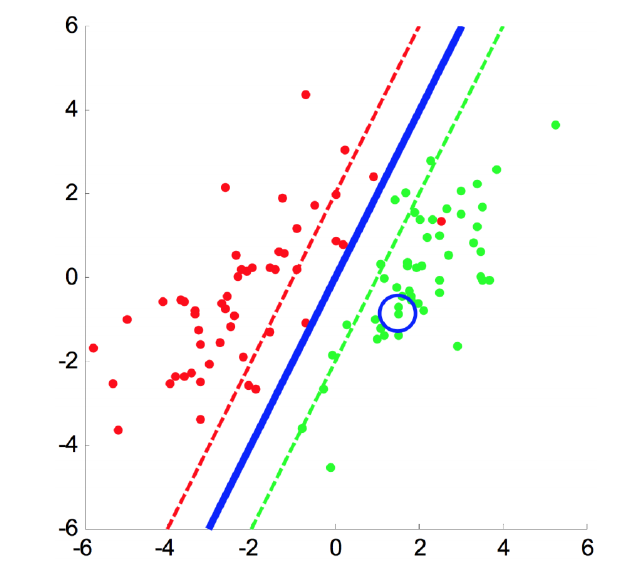
\includegraphics[width=\columnwidth]{SVMcase.png}
		% Create a subtitle for the figure.
		\caption{Example of not linearly separable data}
		% Define the label of the figure. It's good to use 'fig:title', so you know that the label belongs to a figure.
		\label{fig1}
		\end{center}
	\end{figure}\\
To address this problem, we introduce variable $\varepsilon_i \geq 0$, for each $i$, which represents how much example $i$ is on wrong side of margin boundary.
Thus in this lab, we use hinge loss function to evaluate the goodness of our model:
\begin{equation}
\varepsilon_i = max(0,1-y_i(w^Tx_i +b ))
\end{equation} \\
In this lab, the optimization problem then becomes:
\begin{equation}
min (\frac{||w||^2} 2 + \frac C n \sum_{i=1}^n max(0,1-y_i(w^Tx_i +b))
\end{equation} \\
The MSGD method is used to reduce the loss of the model.
\section{Experiments}
\subsection{Dataset}
The experiment uses a9a of LIBSVM Data, including 32561/16281(testing) samples and each sample has 123/123 (testing) features.

\subsection{Implementation}
\center \textbf{Logistic Regression and Batch Stochastic Gradient Descent}\\

Firstly,load the training set and validation set. Then,To initialize logistic regression model parameter, I initialize my w with a matrix whose all entries are zero. Thirdly, I determine the batch size(1024) and randomly take some samples,calculate gradient G toward loss function from partial samples and use the MSGD optimization method to update the parametric model
Finally, to evaluate the model I select the appropriate threshold, mark the sample whose predict scores greater than the threshold as positive, on the contrary as negative, predict under validation set and get the loss on validation set.
	\begin{figure}[!hbt]
		% Center the figure.
		\begin{center}
		% Include the eps file, scale it such that it's width equals the column width. You can also put width=8cm for example...
		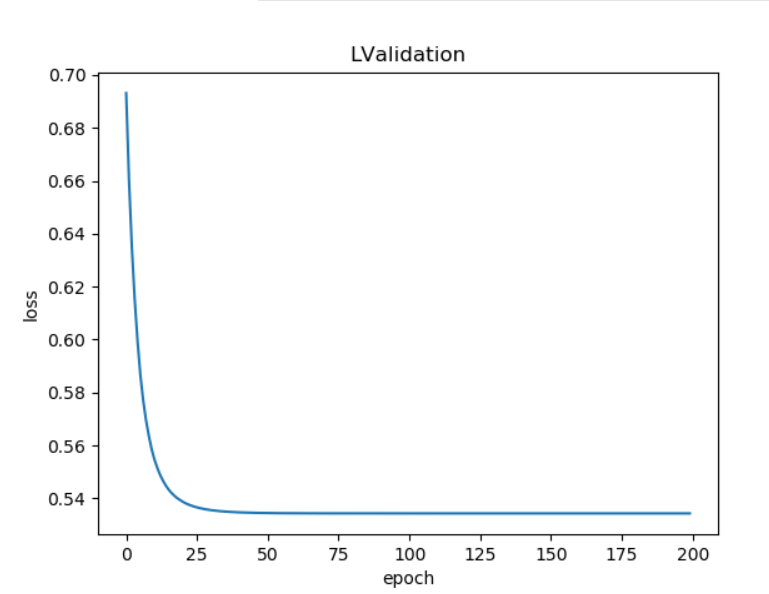
\includegraphics[width=\columnwidth]{logistic.png}
		% Create a subtitle for the figure.
		\caption{Lvalidation chage of logistic regression}
		% Define the label of the figure. It's good to use 'fig:title', so you know that the label belongs to a figure.
		\label{fig2}
		\end{center}
	\end{figure}\\
\center \textbf{Linear Classification and Batch Stochastic Gradient Descent}\\
After loading the training set and validation set I initialize SVM model parameters w into a matrix of zeros. The loss function that I select has been introduced above. Next I choose 1024 as my batch size and randomly take some samples,calculate gradient G toward loss function from partial samples. MSGD optimization is the following step and finally I get the result graph as below:
\begin{figure}[!hbt]
		% Center the figure.
		\begin{center}
		% Include the eps file, scale it such that it's width equals the column width. You can also put width=8cm for example...
		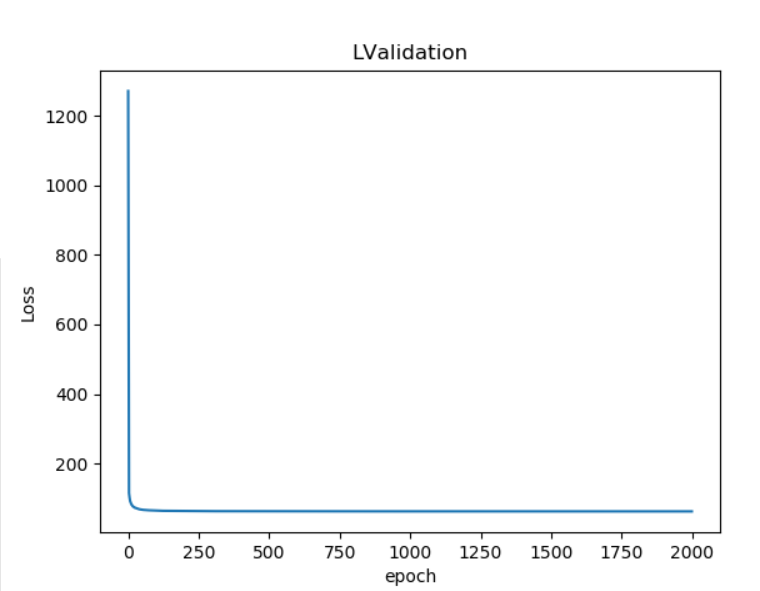
\includegraphics[width=\columnwidth]{SVM.png}
		% Create a subtitle for the figure.
		\caption{Lvalidation chage of SVM.}
		% Define the label of the figure. It's good to use 'fig:title', so you know that the label belongs to a figure.
		\label{fig3}
		\end{center}
\end{figure}
\par
\quad \\


\section{Conclusion}
	This lab is quite challenging compared to lab1, especially in the SVM part. After constructing my naive model, I found that my model has a problem that a pal told me. The problem is that after training, my model can simply mark all the testing set data $x_i$ into $-1$. Days after, my classmate tells me that I may ignore the C constant in the model. Then I make some researches online and adjust my C in the model, the problem is addressed! This lab is fabulously inspiring

% Your document ends here!
\end{document}
